\documentclass[thesis.tex]{subfile}

\chapter{Implementation}
\label{ch:implementation}

% TODO: rewrite this para
We discuss our implementation of time-tiling in detail.
The latter extends the former, while depending crucially on an initial skewing transformation.
We examine the safeguards necessary to prevent errors caused by improper skewing.
Finally, we consider the implications on sparse loops, one of Devito's raisons d'\^etre.

As outlined in Section~\ref{sec:bg-time-tiling}, we implement time-tiling in two stages: skewing in the DSE (Section~\ref{sec:skewing}), and tiling in the DLE (Section~\ref{sec:time-tiling}).


\section{Skewing}
\label{sec:skewing}
A loop nest comprises several nested loops, each with its own loop variable.
We may assume the outermost loop holds the time variable without loss of generality.\footnote{Otherwise, ignore any outer loops.}
In our implementation, inner loop variables are increased by a factor of time, and the index accesses of that variable are decreased by the same factor in the loop body (Figures~\ref{lst:skewing-simple} and~\ref{fig:skewed-loops-skewed-space}).
In this way, all accesses refer to the same data as before the transformation, ensuring its validity.

\begin{figure}[!ht]
\begin{lstlisting}
for (int t = t_s; t < t_e; t++)
  for (int x = x_s; x < x_e; x++)
    A[t][x] = A[t-1][x-1] + A[t-1][x+1];

for (int t = t_s; t < t_e; t++)
  for (int x = x_s + t; x < x_e + t; x++)
    A[t][(x-t)] = A[t-1][(x-t)-1] + A[t-1][(x-t)+1];
\end{lstlisting}
	\caption{The code transformation of skewing: an unskewed loop, and a skewed version of the same loop. Note that all index accesses still refer to the same values.}
	\label{lst:skewing-simple}
\end{figure}

\begin{figure}[!ht]
\centering
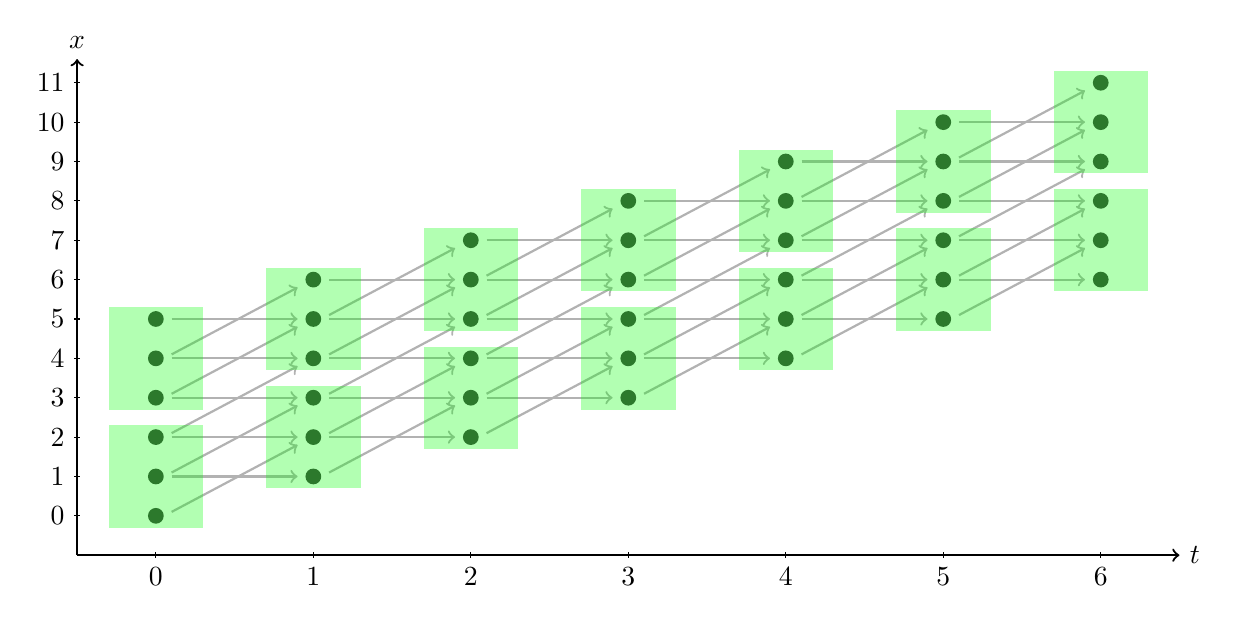
\begin{tikzpicture}
\draw[thick,->] (-1,-.5) -- (13,-.5) node[right]{$t$};
\draw[thick,->] (-1,-.5) -- (-1,5.8) node[above]{$x$};

\foreach \t in {0,1,2,3,4,5,6}
\foreach \x in {0,1,2,3,4,5}
\fill[darkgray] (\t*2,\x/2+\t/2) circle (0.1);

\foreach \t in {0,1,2,3,4,5}
\foreach \x in {1,2,3,4,5}
\draw[thick,->,gray!60] (\t*2+.2,\x/2+\t/2) -- (\t*2+1.8,\x/2+\t/2);

\foreach \t in {0,1,2,3,4,5}
\foreach \x in {0,1,2,3,4}
\draw[thick,->,gray!60] (\t*2+.2,\x/2+\t/2+.05) -- (\t*2+1.8,\x/2+\t/2+.9);

\foreach \t in {0,1,2,3,4,5,6}
\foreach \x in {0,3}
\fill[green,opacity=0.3] (\t*2-.6,\x/2+\t/2-.15) rectangle (\t*2+.6,\x/2+\t/2+1.15);

\foreach \t in {0,1,2,3,4,5,6}
\draw (\t*2,1pt-.5cm) -- (\t*2,-1pt-.5cm) node[anchor=north] {$\t$};
\foreach \x in {0,1,2,3,4,5,6,7,8,9,10,11}
\draw (1pt-1cm,\x/2) -- (-1pt-1cm,\x/2) node[anchor=east] {$\x$};
\end{tikzpicture}
\caption{A skewed iteration space. Dependencies between blocks have not changed, and interchange is \emph{not} valid. (Skewed) tiles included for reference.}
\label{fig:skewed-loops-skewed-space}
\end{figure}

Note that skewing \emph{does not} change the execution order of the loops, nor does it change the structure of the loop nest.

\subsection{Common sub-expression elimination}
As skewing is merely a substitution of indices and loop bounds, we do not change the expressions.
Since arithmetic on floats is generally non-commutative, we especially wish to avoid changing the structure of expressions, to simplify testing of the code.

In particular, we ensure than skewing is performed \emph{before} CSE occurs, to avoid expansion during skewing.
CSE does not remove the skew, as it is partially applied in the loop header, and partially in the expression (see Figure~\ref{lst:skewing-simple}).

\subsection{Implementation}
This was a straightforward substitution in the Devito symbolic engine, exactly as described above.
We iterate over the dimensions, first identifying the time dimension, then adding the offset to each inner space dimension.
We then replace every reference to the space dimension variable with a similar reference, subtracting the offset.

If there is no time dimension, no skewing is applied, as time-tiling would not be relevant.


\section{Time-tiling}
\label{sec:time-tiling}
As we noted in the previous section, skewing has not changed the execution order: when applying the tiling transformation, we now have skewed tiles on a skewed iteration space (Figure~\ref{fig:skewed-loops-skewed-space}).
We now need to `straighten' the tiles by aligning the loop bounds.
All the transformations in this section pertain to tiling, and they are performed in the Devito loop engine.


\subsection{Aligning the loop bounds}
We need to modify the tiling transformation slightly to make the interchange valid.
This was explored in Section~\ref{sec:bg-time-tiling}.
As this alignment was achieved alongside bounding for valid array accesses (detailed in the next section), Figures~\ref{lst:skew-straight} and~\ref{fig:skew-straight} are for illustrative purposes only.

\begin{figure}[!ht]
\begin{lstlisting}
for (int t_blk = t_s; t_blk < t_e; t_blk += t_blk_size)
  for (int t = t_blk; t < min(t_e, t_blk + t_blk_size); t++)
    for (int x_blk = x_s; x_blk < x_e + t_e; x_blk += x_blk_size)
      for (int x = x_blk; x < min(x_e + t_e, x_blk + x_blk_size); x++)
        A[t][(x-t)] = A[t-1][(x-t)-1] + A[t-1][(x-t)+1];
\end{lstlisting}
	\caption{Code which has been tiled following a skewing transformation. This code contains invalid array accesses.}
	\label{lst:skew-straight}
\end{figure}

\begin{figure}[!ht]
	\centering
	\begin{tikzpicture}
	\draw[thick,->] (-1,-.5) -- (13,-.5) node[right]{$t$};
	\draw[thick,->] (-1,-.5) -- (-1,5.8) node[above]{$x$};
	
	\foreach \t in {0,1,2,3,4,5,6}
	\foreach \x in {0,1,2,3,4,5,6,7,8,9,10,11}
	\draw (\t*2,\x/2) node[cross=2.4,red]{};
	
	\foreach \t in {0,1,2,3,4,5,6}
	\foreach \x in {0,1,2,3,4,5}
	\fill[darkgray] (\t*2,\x/2+\t/2) circle (0.1);
	
	\foreach \t in {0,1,2,3,4,5}
	\foreach \x in {1,2,3,4,5}
	\draw[thick,->,darkgray!60] (\t*2+.2,\x/2+\t/2) -- (\t*2+1.8,\x/2+\t/2);
	
	\foreach \t in {0,1,2,3,4,5}
	\foreach \x in {0,1,2,3,4}
	\draw[thick,->,darkgray!60] (\t*2+.2,\x/2+\t/2+.05) -- (\t*2+1.8,\x/2+\t/2+.9);
	
	\foreach \t in {0,1,2,3,4,5,6}
	\foreach \x in {0,3,6,9}
	\fill[green,opacity=0.3] (\t*2-.6,\x/2-.15) rectangle (\t*2+.6,\x/2+1.15);
	
	\foreach \t in {0,1,2,3,4,5,6}
	\draw (\t*2,1pt-.5cm) -- (\t*2,-1pt-.5cm) node[anchor=north] {$\t$};
	\foreach \x in {0,1,2,3,4,5,6,7,8,9,10,11}
	\draw (1pt-1cm,\x/2) -- (-1pt-1cm,\x/2) node[anchor=east] {$\x$};
	\end{tikzpicture}
	\caption{Straightened tiles on a skewed iteration space. Invalid array accesses indicated by crosses.}
	\label{fig:skew-straight}
\end{figure}


\subsection{Min/max bounds for valid array accesses}
Since a skewed iteration space is not rectangular (or in general, not a hypercube), valid array accesses over a space variable will not be valid for the same values between time iterations (as seen the previous section).
As it is not feasible to generate a remainder loop for each time iteration and choice of space dimension,\footnote{This would require at least \(\sum_{m=1}^{n} \binom{n}{m} = 2^n \) remainder loop nests, where there are \(n\) spatial dimensions -- one for each choice of dimensions.} we bound the inner loops using the \texttt{min} and \texttt{max} functions.

\begin{figure}[!ht]
\begin{lstlisting}
for (int t_blk = t_s; t_blk < t_e; t_blk += t_blk_size)
  for (int t = max(t_s, t_blk);
           t < min(t_e, t_blk + t_blk_size); t++)
    for (int x_blk = x_s; x_blk < x_e + t_e; x_blk += x_blk_size)
      for (int x = max(x_s + t, x_blk);
               x < min(x_e + t, x_blk + x_blk_size); x++)
        A[t][(x-t)] = A[t-1][(x-t)-1] + A[t-1][(x-t)+1];
\end{lstlisting}
	\caption{We add lower bounds for each of the inner (e.g. \texttt{x}, not \texttt{x\_blk}) variables, and we change the upper bounds for the spatial dimensions to be bounded by \texttt{x\_e + t}, instead of \texttt{x\_e + t\_e}. This prevents out of bounds accesses in the lower and upper triangular regions of Figure~\ref{fig:skewing-bounded} respectively.}
	\label{lst:skewing-bounded}
\end{figure}

\begin{figure}[!ht]
\centering
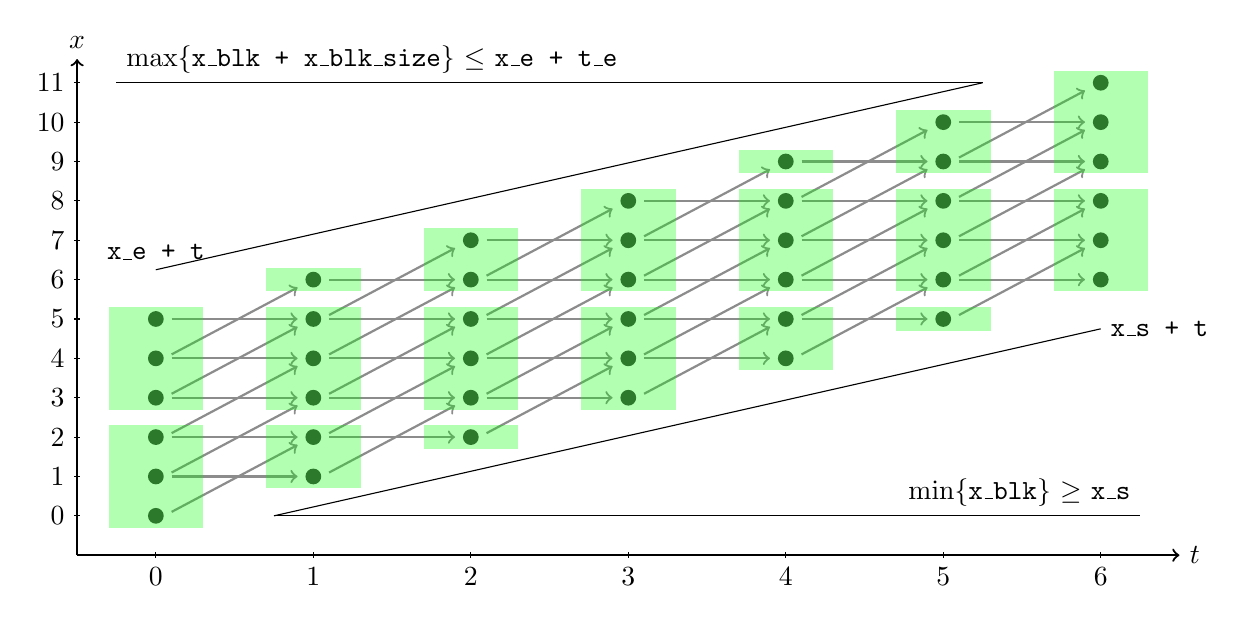
\begin{tikzpicture}
\draw[thick,->] (-1,-.5) -- (13,-.5) node[right]{$t$};
\draw[thick,->] (-1,-.5) -- (-1,5.8) node[above]{$x$};

% triangles
\draw (1.5,0) -- (12.5,0) node[anchor=south east] {min\{\texttt{x\_blk}\} \(\ge\) \texttt{x\_s}};
\draw (1.5,0) -- (12,2.375) node[anchor=west] {\texttt{x\_s + t}};
\draw (10.5,11/2) -- (-.5,11/2) node[anchor=south west] {max\{\texttt{x\_blk + x\_blk\_size}\} \(\le\) \texttt{x\_e + t\_e}};
\draw (10.5,11/2) -- (0,3.125) node[anchor=south] {\texttt{x\_e + t}};

\foreach \t in {0,1,2,3,4,5,6}
\foreach \x in {0,1,2,3,4,5}
\fill[darkgray] (\t*2,\x/2+\t/2) circle (0.1);

\foreach \t in {0,1,2,3,4,5}
\foreach \x in {1,2,3,4,5}
\draw[thick,->,darkgray!60] (\t*2+.2,\x/2+\t/2) -- (\t*2+1.8,\x/2+\t/2);

\foreach \t in {0,1,2,3,4,5}
\foreach \x in {0,1,2,3,4}
\draw[thick,->,darkgray!60] (\t*2+.2,\x/2+\t/2+.05) -- (\t*2+1.8,\x/2+\t/2+.9);

\foreach \t in {0,1,2,3} \foreach \x in {3}
\fill[green,opacity=0.3] (\t*2-.6,\x/2-.15) rectangle (\t*2+.6,\x/2+1.15);

\foreach \t in {3,4,5,6} \foreach \x in {6}
\fill[green,opacity=0.3] (\t*2-.6,\x/2-.15) rectangle (\t*2+.6,\x/2+1.15);

\foreach \t in {0} \foreach \x in {0}
\fill[green,opacity=0.3] (\t*2-.6,\x/2-.15) rectangle (\t*2+.6,\x/2+1.15);

\foreach \t in {6} \foreach \x in {9}
\fill[green,opacity=0.3] (\t*2-.6,\x/2-.15) rectangle (\t*2+.6,\x/2+1.15);

\foreach \t in {1} \foreach \x in {1}
\fill[green,opacity=0.3] (\t*2-.6,\x/2-.15) rectangle (\t*2+.6,\x/2+.65);

\foreach \t in {2} \foreach \x in {6}
\fill[green,opacity=0.3] (\t*2-.6,\x/2-.15) rectangle (\t*2+.6,\x/2+.65);

\foreach \t in {4} \foreach \x in {4}
\fill[green,opacity=0.3] (\t*2-.6,\x/2-.15) rectangle (\t*2+.6,\x/2+.65);

\foreach \t in {5} \foreach \x in {9}
\fill[green,opacity=0.3] (\t*2-.6,\x/2-.15) rectangle (\t*2+.6,\x/2+.65);

\foreach \t in {2} \foreach \x in {2}
\fill[green,opacity=0.3] (\t*2-.6,\x/2-.15) rectangle (\t*2+.6,\x/2+.15);

\foreach \t in {1} \foreach \x in {6}
\fill[green,opacity=0.3] (\t*2-.6,\x/2-.15) rectangle (\t*2+.6,\x/2+.15);

\foreach \t in {5} \foreach \x in {5}
\fill[green,opacity=0.3] (\t*2-.6,\x/2-.15) rectangle (\t*2+.6,\x/2+.15);

\foreach \t in {4} \foreach \x in {9}
\fill[green,opacity=0.3] (\t*2-.6,\x/2-.15) rectangle (\t*2+.6,\x/2+.15);

\foreach \t in {0,1,2,3,4,5,6}
\draw (\t*2,1pt-.5cm) -- (\t*2,-1pt-.5cm) node[anchor=north] {$\t$};
\foreach \x in {0,1,2,3,4,5,6,7,8,9,10,11}
\draw (1pt-1cm,\x/2) -- (-1pt-1cm,\x/2) node[anchor=east] {$\x$};
\end{tikzpicture}
\caption{Straightened tiles on a skewed iteration space, with restrictions to valid accesses. The lower triangular reason corresponds to the \texttt{max} bound in Figure~\ref{lst:skewing-bounded}, restricting accesses by the greater of the two lines. Likewise the upper triangular reason corresponds to the \texttt{min} bound.}
\label{fig:skewing-bounded}
\end{figure}

At the same time, it makes sense for this approach to supersede the remainder loops detailed in Section~\ref{sec:remainder-loops} which generate remainder iterations.
This is valid because every array access is valid under the new bounds.
We can therefore extend the iteration space of the outermost (tiling) loop to the full extent of the skewed iteration space.
This would have previously resulted in out-of-bounds accesses as bounding did not occur.

Figures~\ref{lst:skewing-bounded} and~\ref{fig:skewing-bounded} combine skewing and min/max bounding.

\subsection{Implementation}
Unlike skewing implemented in the DSE, tiling was not done through a simple substitution of variables.
Instead, the visitor pattern was used to manipulate Devito's internal representation of the loop structure.

Together, the following paragraphs explain this design decision.

\paragraph{OpenMP and \texttt{fmax}}
While we have used the \texttt{max} function in examples, the only similar function in C, which Devito generates, is \texttt{fmax}.
However, it is known that we are unable to use \texttt{fmax} in a loop header when the loop is parallelised under OpenMP due to scoping and optimisation problems~\cite{openmp-fmax}.

\paragraph{Loop nest structure}
Each tiled loop would be tiled into two loops: an inner \texttt{x} loop, and an outer \texttt{x\_blk} loop, for the tiles.
Substitution would be tricky, as the body of each loop would have to be copied and substituted in turn.
Only then could the loops be interchanged.

\paragraph{Perfect loop nests}
Definition. A \emph{perfect loop nest} is a loop which fulfilling this condition: its body contains either a perfect loop nest, or only non-loop statements.

\begin{figure}[!ht]
\begin{lstlisting}
for (int x_blk = x_s; x_blk < x_e + t_e; x_blk += x_blk_size)
  int x_lb = fmax(x_s + t, x_blk);
  int x_ub = fmin(x_e + t, x_blk + x_blk_size);
  for (int x = x_lb; x < x_ub; x++)
    A[t][(x-t)] = A[t-1][(x-t)-1] + A[t-1][(x-t)+1];
\end{lstlisting}
	\caption{Bounds hoisted out of the loop header.}
	\label{lst:hoist-bounds}
\end{figure}

\paragraph{Direct construction of loop nests}
In Devito's existing implementation of spatial tiling, loops were tiled with a function designed to manipulate perfect loop nests.
Each loop would be duplicated, adjusting the bounds on the resultant loop, then composed, along with the body of the innermost loop.
However, as it proved impossible to insert the \texttt{fmax} function directly into the loop header, it was necessary to hoist computation of the bounds to before each loop (Figure~\ref{lst:hoist-bounds}).
As this did not resemble a perfect loop nest,\footnote{Note that the control-flow graph of the program would not change under hoisting this expression, and the code motion is legal as the value is loop-invariant.} the approach of composition failed.

\subsubsection{Visitor pattern}
Given the above constraints, we found that the visitor pattern would be the most practical solution to constructing a new tiled loop nest.
This allowed for easy propagation of loop properties, offsets to the upper and lower bounds, and a clear distinction between the parallelisable inner loops, and the sequential outer tile loops.


\section{Test suite}
Devito has an extensive test suite, which we endeavoured not to break while implementing time-tiling.
In particular, the existing tests used for spatial tiling were helpful, as they provided a benchmark for the correct tiling behaviour.

We extended the test suite, verifying the following:

\begin{itemize}
	\item Skewing must not change the numerical results.
	\item Spatial tiling behaves as it did before.
	\item Time-tiling with skewing produces the same results as non-tiled code. This would be equal to the spatially-tiled code.
\end{itemize}


\section{Auto-tuning}
\label{sec:autotune}

% TODO: rewrite
Time-tiling introduces two parameters that can be tuned: the skewing factor, and time tile size.

Since time-tiling had not been implemented in Devito before, it was decided that the auto-tuner should try all reasonable time tile sizes.
It was modified for this behaviour, as well as minor changes to try additional specific combinations, such as trying the maximum block size for the innermost dimension.

We have not extended the auto-tuner to try different skewing factors as we hope to include it in the evaluation.
Therefore, auto-tuning will be performed for the relevant skewing factors.
Manually varying the skewing factor is not an undue burden, as there are very few plausible skewing factors.

\section{Further work}
The implementation work that remains can be divided into several tasks:

\begin{description}
	\item[Time-tiling] This is essentially complete. Some outstanding items:
	\begin{itemize}
		\item Removal of `empty' blocks -- trivial; does not affect correctness but might produce speedup\footnote{CLooG does it, but one has difficulty imagining that there will indeed be a noticeable speedup}
		\item Making this work with time buffering -- some reasoning about skewing factor required
		\item Test cases -- more can be added
		\item Removal of test cases assuming a remainder loop structure
		\item Verification that a given skewing factor is valid -- this should be very easy as Devito knows all about the stencil
	\end{itemize}

	\item[DSE aggressive mode] Currently, no reason to suppose that this cannot work with \texttt{min}-bounded instead of remainder loops. Need to prove/disprove this, and make it work. In particular, we must examine the references made to certain variables.\footnote{Of particular interest are \texttt{blockshape} (the tile size) and dimension extents (e.g.~symbolic extent vs offsets).}

	\item[Sparse loop interpolation] Gather more context and understanding of the problem will be important for reasoning about how this affects time-tiling. Ideally, eventually a proof of what it does/why it does not.

	\item[Detection of when to apply skewing and calculation of the skewing factor] Whether time-tiling is an appropriate optimisation, for a given stencil. Entirely beyond the scope of this work.

	\item[Vectorisation and time-tiling] Suspect something is going wrong, full length of inner dimension are slower than non-blockinner trials. Remark: because of AT fail, probably having \texttt{z\_bs = 8}.
\end{description}
